% Preamble

\documentclass[../main.tex]{subfiles}
\graphicspath{{\subfix{../images/}}}

\begin{document}



\section{Introduction}

Satellite communication system have been one of the most important advances in twentieth century. On one hand, they are a powerful alternative to other systems, like HF radio links or submarine wires, since they get to provide coverage for large surfaces (a GEO satellite covers $1/3$ of Earth surface).

However, communication and control equipment must be highly reliable since it can be impossible to be repaired. Satellites are exposed to high radiation conditions and a virtually limited life and a high risk of being destroyed in launching.

In general, satellite communication systems are economically viable. They are not a substitute but a complement to other system. For example, international telephony works with both submarine wires and satellites.

\section{Satellite systems key aspects}

\subsection{Services}

Satallite systems provide a series of services to complement terrestrial communication systems:
\begin{itemize}
	\item Fixed service: Links between two fixed terrestrial points. It is used for telephony, TV and data.
	\item Mobile service: It allows communications with one or more mobile points. It is useful for navy, terrestrial and aeronautical purposes.
	\item Broadcasting service: It allows the access to one or more fixed points through spread terminals. It is used to broadcast audio and images.
	\item Radiolocalization services.
	\item {
		Earth exploring services:
		\begin{itemize}
			\item Meteorology.
			\item Geodesy: Study of Earth shape, dimensions and gravitational field. It is useful for the making of topographic maps.
			\item Resource search.
		\end{itemize}
	}
	\item Space scan services: Telescopes and radio-telescopes.
	\item Services between satellites.
\end{itemize}

\subsection{Architecture of satellite communication systems}

Satellite systems are implemented through the following elements:
\begin{itemize}
	\item Electric Ground Support Equipment (EGSE): Groung system for transmission and reception of base-band signal. It carries out modulation, conversion to Intermediate Frequency (IF), conversion to Radio Frequency RF, amplification and transmission. High transmission power and directivity are required.
	\item Uplink and downlink: Signal propagates through free space. It attenuates with the square of frequency and distance. It is also important to take care with atmosphere and rain, which are sources of attenuation.
	\item {
		Satellite: It assumes different roles such as, repeater station, amplifier, band change and retransmission. For that purpose, it is equiped with different systems:
		\begin{itemize}
			\item Reception: Antenna, filter, and low noise amplifier.
			\item Transponder: It carries out frequency conversion and amplification.
			\item Switching: It consists on routing and transponder selection.
			\item Transmission: Power amplification, filter and antenna.
		\end{itemize}
	}
\end{itemize}

\begin{figure}[H]
	\centering
	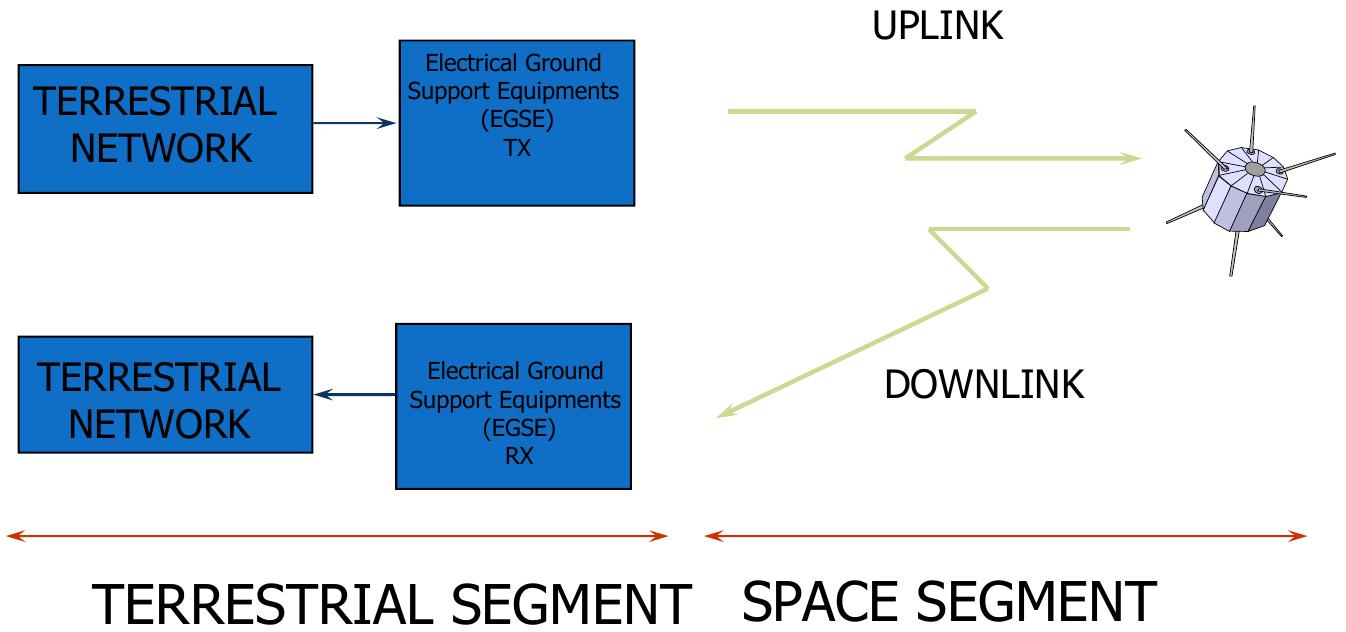
\includegraphics[
		width=14cm,
		%height=15cm
	]{images/Tema 5/Architecture.png}
	\caption{
		\label{fig:unit5_Architecture}
		Satellite systems architecture
	}
\end{figure}

\subsection{Specifications of satellite communication systems}

The design of a satellite system depends on radio frequency and geometrical aspects:
\begin{itemize}
	\item Orbit: Most applications use Geostationary Orbit (GEO). However, for Personal Communications Systems (PCS) other orbits are being used such as Medium Earth Orbit (MEO) and Low Earth Orbit (LEO).
	\item Coverage: Depending on orbit and antenna system, satellites can provide a global beam ($1/3$ of Earth surface), local beam (up to 800 $km^2$) or beamforming (intermediate coverage, such as a country, an island, etc.).
	\item Connectivity: Capacity of linking by using the different ground stations. It depends on the satellite’s capacity and multiple access techniques.
	\item Multiple access and shared access: The way the satellite is shared, typically FDMA, TDMA or CDMA.
	\item Frequency band and bandwidth: Different frequency bands are used depending on service and availability (originally band C (6/4 GHz), later band Ku (14/11 GHz), Ka, \ldots). Higher frequencies means worse propagation. Satellite must implement reuse tecnniques (separating beams at the same frequency, polarization, \ldots), signal processing and efficient modulation (more channels for a given bandwidth).
	\item Power: Satellite must carry out a trade off between distance to Earth and limitation on the on-board energy. Solar panels and Travelling Wave Tube Amplifiers (TWTA) provide enough power now. Current limitations are due to interferences from other satellites and EGSEs.
\end{itemize}

\subsection{Geometry of satellite communication systems}

\subsubsection{Orbits}

Orbits are a key element in the design of a satellite system. They are driven by Kepler laws and gravitaty. The path is conical and the type depends on the energy of the system. The choice depends on the coverage, the applications, economical issues, etc. It is a limited resource since different satellite provides compete for them.

There are two basic orbit types:
\begin{itemize}
	\item {
		Geostationary Orbit (GEO): 36000 km. Circular orbit and equatorial. Null inclination (slope). Revolution period equals an Earth period (synchronous). Satellite is always visible (except during eclipses) and does not require (in theory) tracking. GEO covers large areas and allows fixed antennas on Earth. It is used to implement fixed services, mobile communications, broadcast services, \ldots Some GEO drawbacks are:
		\begin{itemize}
			\item It requires a high power transmission since distance increments attenuation.
			\item Large aperture antennas.
			\item High altitude regions are not properly covered.
			\item Long delays.
			\item Launching is more expensive.
		\end{itemize}
	}
	\item {
		Oblique orbit: The satellite raises and fall. We have visibility periods. Tracking is very important. Orbits are lower than GEO, so launching is tipically cheaper. It is used to implement mobile services and other applications, even non related with communications. In this class, we include:
		\begin{itemize}
			\item Low Earth Orbit (LEO): 200 km - 3000 km.
			\item Medium Earth Orbit (MEO): 3000 km - 11000 km.
			\item {
				Highly Elliptical Orbit (HEO): Up to 40000 km. In this class is included Molniya orbit:
				\begin{itemize}
					\item Tilted with respect the Equator.
					\item Mostly used by Russia because of the high latitude of its territory.
					\item At the apogee, the speed is much lower than in the perigee.
				\end{itemize}
			}
		\end{itemize}
	}
\end{itemize}

\begin{figure}[H]
	\centering
	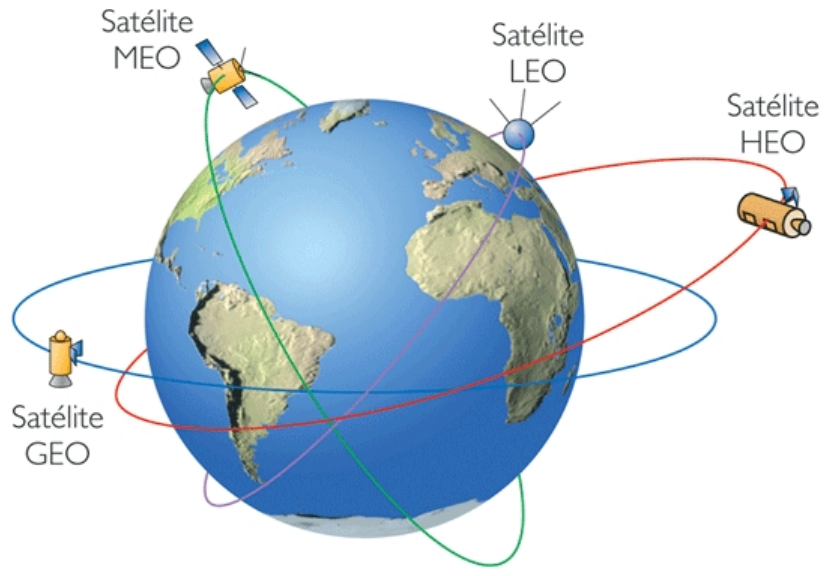
\includegraphics[
		width=8cm,
		%height=15cm
	]{images/Tema 5/Orbits.png}
	\caption{
		\label{fig:unit5_orbits}
		Satellite orbits
	}
\end{figure}

\begin{figure}[H]
	\centering
	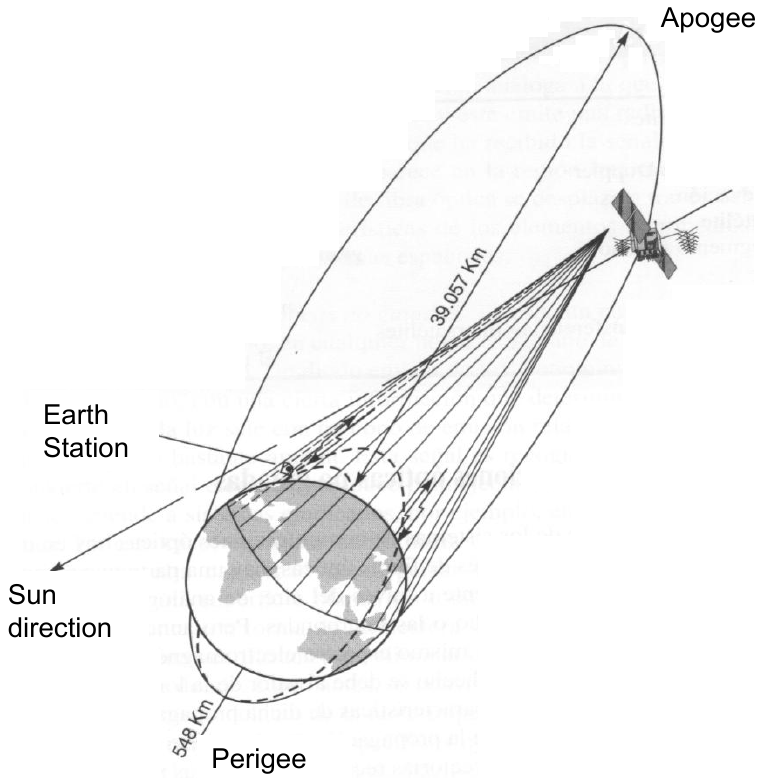
\includegraphics[
		width=9cm,
		%height=15cm
	]{images/Tema 5/Molniya.png}
	\caption{
		\label{fig:unit5_Molniya}
		Molniya orbit
	}
\end{figure}

\subsubsection{Coverage}

A different coverage is provided depending on the Earth antenna elevation:
\begin{itemize}
	\item Geometrical coverage: The Earth area that is visible from the satellite. It is the tangent cone from satellite.
	\item Radio electric coverage: It is lower because antennas need at least $5^{\circ}$ on inclination due to obstacles and noise.
\end{itemize}

\subsubsection{Orientation}

In order to study satellite orientation, we consider the following variables:
\begin{itemize}
	\item {
		Equivalent Earth radius:
		$$
			R = 6377 [km]
		$$
	}
	\item Satellite high: $h$
	\item {
		Orbit radius:
		$$
			a = R + h
		$$
	}
	\item Terrestrial pole: $P$
	\item Longitude origin (positive values for East and negative values for West): $Q$
	\item {
		Greenwich Meridian:
		$$
			PQ = (r, \varphi, \lambda) = (R, 0, \lambda)
		$$
	}
	\item {
		Satellite coordinates (spherical):
		$$
			S_{sphe} = (r, \varphi, \lambda) = (R + h, \varphi_1, 0)
		$$
	}
	\item {
		Satellite coordinates (Cartesian):
		$$
			S_{Cart} = (x_S, y_S, z_S) = (R + h, 0, 0)
		$$
	}
	\item {
		Sub-satellite point:
		$$
			S' = (r, \varphi, \lambda) = (R, \varphi_1, 0)
		$$
	}
	\item {
		Ground station coordinates (spherical):
		$$
			E_{sphe} = (r, \varphi, \lambda) = (R, \varphi_0, \lambda)
		$$
	}
	\item {
		Ground station coordinates (Cartesian):
		$$
			E_{Cart} = (x_E, y_E, z_E) =
			(R \cdot \cos (\varphi) \cdot \cos (\lambda), R \cdot \sin (\varphi) \cdot \cos (\lambda), R \cdot \sin (\lambda) )
		$$
	}
	\item {
		Distance from satellite to ground station:
		$$
			ES = d =
			\sqrt{ (x_S - x_E )^2 + y_{E}^2 + z_{E}^2 } =
			\sqrt{ ( R + h )^2 + R^2 - 2 R \cdot (R+h) \cdot \cos(\varphi) \cdot \cos(\lambda) }
		$$
	}
\end{itemize}

\begin{figure}[H]
	\centering
	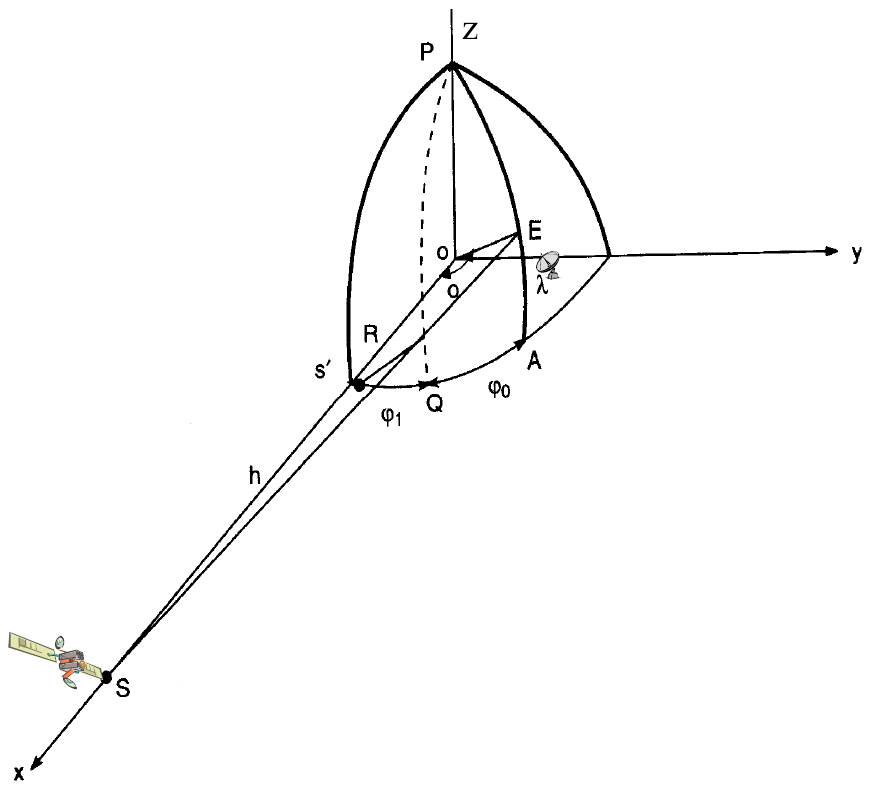
\includegraphics[
		width=10cm,
		%height=15cm
	]{images/Tema 5/Orientation.png}
	\caption{
		\label{fig:unit5_Orientation}
		Orientation
	}
\end{figure}

\subsubsection{View angles}

Some angles must studied:
\begin{itemize}
	\item {
		Elevation angle ($\hat{El}$): From horizontal to satellite direction.
		$$
			\hat{a} = \arccos \left( \cos (\varphi) \cdot \cos (\lambda) \right)
		$$
		$$
			\hat{El} = \arctan \left( \frac {\cos (\hat{a}) - \frac{R}{R+h}} {\sin (\hat{a})} \right)
		$$
	}
	\item {
		Azimuth angle ($\hat{A}$): From North to East of horizontal projection of the satellite.
		$$
			\hat{E} = \arctan \left( \frac {\tan (\varphi)} {\sin (\lambda)} \right)
		$$
		$$
			\hat{A} = \left\lbrace \begin{matrix}
				180^{\circ} - \hat{E} & \text{if NW} \\
				180^{\circ} + \hat{E} & \text{if NE} \\
				\hat{E} & \text{if SW} \\
				360^{\circ} - \hat{E} & \text{if SE}
			\end{matrix}\right.
		$$
	}
	\item {
		Central angle (angle created by satellite with ground station seen from Earth centre):
		$$
			\gamma = \arccos \left( \frac {R} {R + h} \cos(\hat{El}) \right) - \hat{El}
		$$
		Some useful relations with central angle:
		$$
			d = h \sqrt{1 + \left( \frac{R}{h} \right)^2 - 2 \frac{R}{h} \cos(\gamma)}
		$$
		$$
			\cos (\hat{El}) =
			\frac {h \cdot \sin (\gamma)} {d} =
			\frac {\sin (\gamma)} {\sqrt{1 + (\frac{R}{h})^2 - 2 \frac{R}{h} \cos(\gamma)}}
		$$
	}
\end{itemize}

\begin{figure}[H]
	\centering
	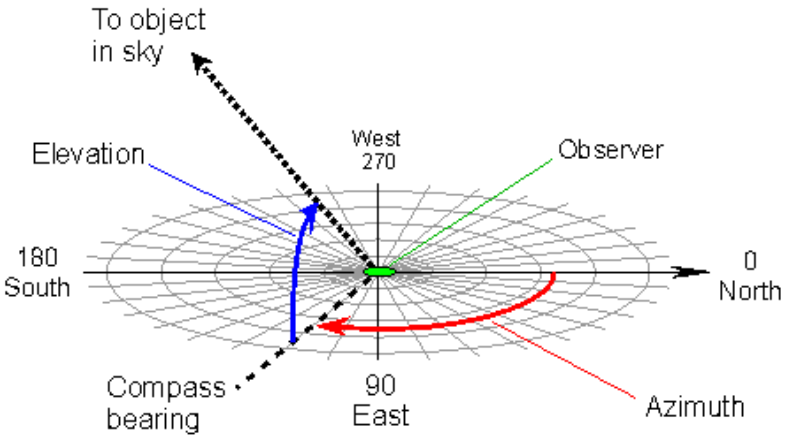
\includegraphics[
		width=10cm,
		%height=15cm
	]{images/Tema 5/View angles.png}
	\caption{
		\label{fig:unit5_view_angles}
		View angles
	}
\end{figure}

\subsubsection{LEO constellations}

Coverage area per satellite is limited, so a large number of satellites for global coverage is needed. They are organized in constellations, LEO orbits, which are circular (polar or tilted) and elliptical.

Basic LEO parameters:
\begin{itemize}
	\item Circular orbits are assumed (eccentricity is 0).
	\item {
		Kepler constant:

		$$
			k = G \cdot m_E = 3.98601352 \cdot 10^5 [km^3/s^2]
		$$
	}
	\item {
		Linear speed:
		$$
			v_s =
			\sqrt {k \cdot \left( \frac {2} {R + h} - \frac {1} {a} \right)} =
			\sqrt {\frac {k} {R + h}}
		$$
	}
	\item {
		Angular speed:
		$$
			\omega_s =
			\frac {v_s} {R + h} =
			\sqrt {\frac {k} {(R + h)^3}}
		$$
	}
	\item {
		Orbit period:
		$$
			T_s =
			2 \pi \sqrt{ \frac {(R + h)^3} {k} }
		$$
	}
	\item {
		Distance from the edge of the coverage:
		$$
			d_{coverage} =
			\sqrt{R^2 + (R + h)^2 - 2 R (R + h) \cos(\gamma)}
		$$
	}
\end{itemize}

\begin{figure}[H]
	\centering
	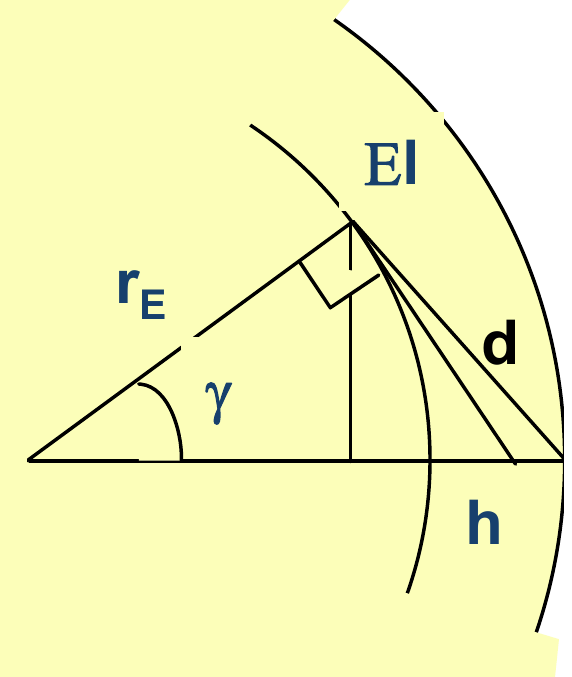
\includegraphics[
		width=5cm,
		%height=15cm
	]{images/Tema 5/LEO parameters.png}
	\caption{
		\label{fig:unit5_LEO_param}
		LEO parameters
	}
\end{figure}

The minimum elevation angle is a very important parameter in these systems. It is the angle the terminal sees the satellite at when it is at the coverage edge. It determines the link availability and it must be taken into account for handovers.

LEO system design consists on a trade-off between number of satellites, delay and losses. In order to estimate the minimum number of satellites we must have in account the region covered by the sphere’s cone:

$$
	S = 2 \pi R^2 \left[ 1 - \cos(\gamma) \right]
$$

\begin{figure}[H]
	\centering
	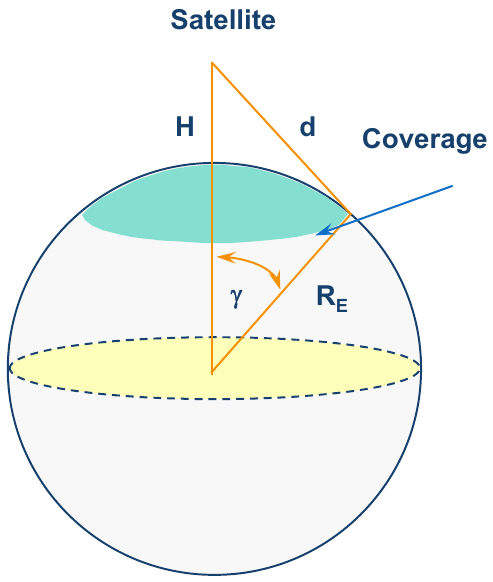
\includegraphics[
		width=6cm,
		%height=15cm
	]{images/Tema 5/Region covered.png}
	\caption{
		\label{fig:unit5_region_LEO}
		Region covered by LEO orbit
	}
\end{figure}

The minimum number of satellites is:

$$
	N = \frac {4 \pi R^2} {S} = \frac {2} {1 - \cos(\gamma)}
$$

\begin{figure}[H]
	\centering
	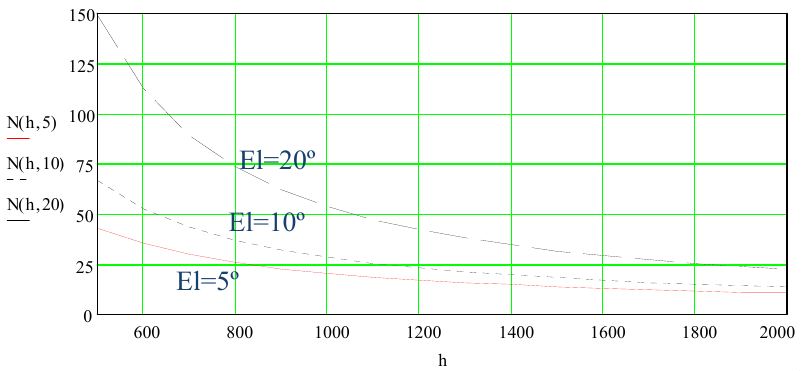
\includegraphics[
		width=14cm,
		%height=15cm
	]{images/Tema 5/Number of satellites.png}
	\caption{
		\label{fig:unit5_number_sat_LEO}
		Minimum number of satellites for different parameters
	}
\end{figure}

For a larger covered area we need a higher number of satellites. If we increase the central angle $\gamma$, we need a lower number of satellites, but that produces delay.

\subsubsection{Eclipses}

Satellites also are affected by eclipses periodically. They must be taken into account for the battery design. We must study apparent Sun movement with respect to the earth and satellite. At solstices, satellites are always illuminated, but at equinoxes there are eclipses of up to 77 minutes a day during several days.

\begin{figure}[H]
	\centering
	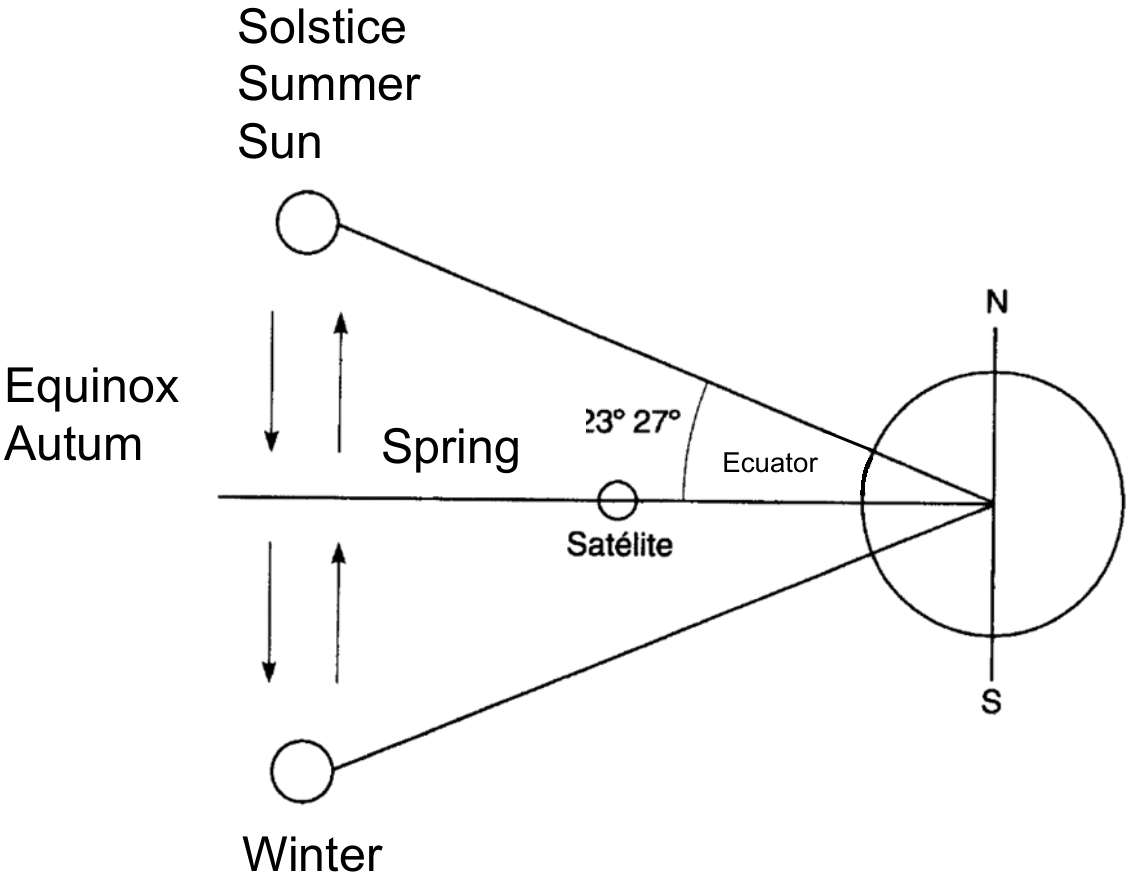
\includegraphics[
		width=10cm,
		%height=15cm
	]{images/Tema 5/Eclipses 1.png}
	\caption{
		\label{fig:unit5_Eclipses_1}
		Eclipses 1
	}
\end{figure}

\begin{figure}[H]
	\centering
	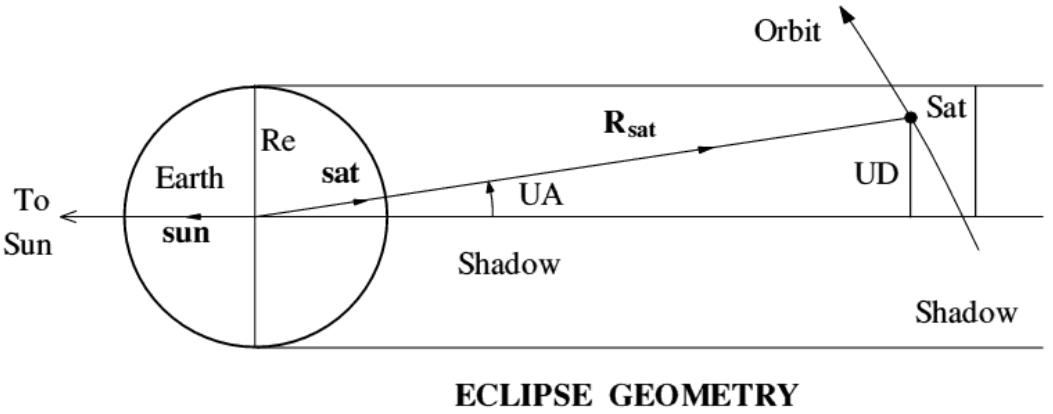
\includegraphics[
		width=10cm,
		%height=15cm
	]{images/Tema 5/Eclipses 2.png}
	\caption{
		\label{fig:unit5_Eclipses_2}
		Eclipses 2
	}
\end{figure}

\begin{figure}[H]
	\centering
	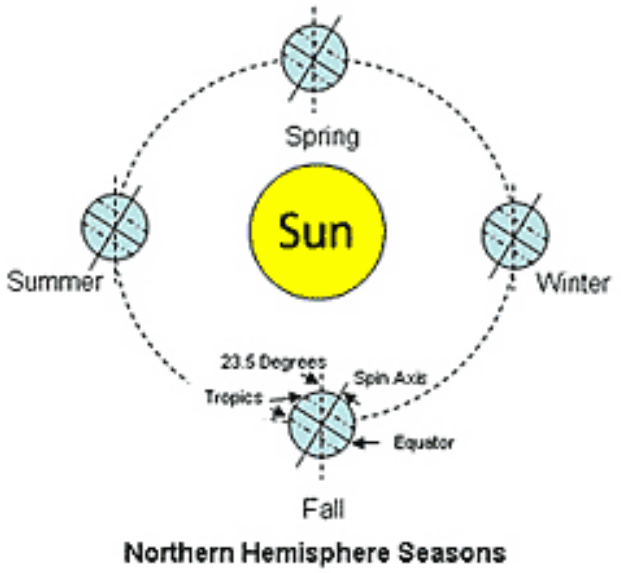
\includegraphics[
		width=10cm,
		%height=15cm
	]{images/Tema 5/Eclipses 3.png}
	\caption{
		\label{fig:unit5_Eclipses_3}
		Eclipses 3
	}
\end{figure}

\subsubsection{Solar interference}

A Sun outage occurs two times at a year depending on the longitude and the latitude. The interference duration is inverse to the antenna size and frequency. Besides, the antenna $T_{eq}$ dramatically increases up to 50000 K, with an antenna of aperture to the apparent sun diameter (32 minutes).

\subsection{Space segment}

\subsubsection{Introduction}

Satellite space element can be studied in two different parts:
\begin{itemize}
	\item {
		Platform: Auxiliary subsystems and structures that are needed to complete the satellite mission although they are not involved into it. In this category, we can highlight:
		\begin{itemize}
			\item Structure sub-system.
			\item Termal control.
			\item Propulsion sub-system.
			\item Altitude and Orbit Control Sub-system (AOCS).
			\item Telemetry, Tracking and Command (TTC) sub-system.
			\item Energy sub-system.
			\item Antenna open up.
		\end{itemize}
	}
	\item {
		Payload: These are the instruments for accomplishing the mission. For example, in the case of communications satellite, these are the transponders and antennas for transmission and reception. We distinguish systems for two types of satellites:
		\begin{itemize}
			\item {
				Analog satellite: It carries out signal reception, amplificacation and frequency conversion. For those purposes, they dispose of:
				\begin{itemize}
					\item Band pass filter.
					\item Tunnel diode amplifier.
					\item Local oscillator.
					\item Amplifier.
					\item High Power Amplifier with TWT.
				\end{itemize}
			}
			\item {
				Digital satellite: It manages signal modulation and a multiple access technique, TDMA (single carrier). There are two possible configurations:
				\begin{itemize}
					\item Frequency conversion and amplification: No demodulation  is carried out (similar to analog satellites). They are called transparent satellites.
					\item Frequency conversion and processing: Demodulation to Base Band (BB), where errors can be corrected or, at least, detected) They are called On Board Processing (OBP) regenerative satellites.
				\end{itemize}
				Main performance measurement is energy per bit to noise density ratio:

				$$
					\frac {E_b} {N_0} = \frac {C} {N} \frac {B} {R_b} = \frac {C} {N_0} \frac {1} {R_b}
				$$

				Where $R_b$ is the binary data rate and c the carrier level.
			}
		\end{itemize}
	}
\end{itemize}

\begin{figure}[H]
	\centering
	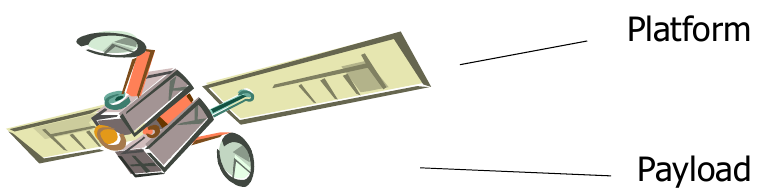
\includegraphics[
		width=10cm,
		%height=15cm
	]{images/Tema 5/Space segment.png}
	\caption{
		\label{fig:unit5_space_segment}
		Space segment
	}
\end{figure}

\subsubsection{Transponder}

The function of transponder is frequency conversion and signal amplification. Transponder bandwidth depends on signals and multiple access techniques. Its main characteristics are:
\begin{itemize}
	\item Flat amplitude response in frequency, working in the linear zone.
	\item Constant group delay.
	\item Linearity in response:
	\item $BO = \frac {P_i} {P_o}$
\end{itemize}

Transponders can be regenerative:
\begin{itemize}
	\item They avoid non linear degradation.
	\item UL and DL adaptation.
	\item The demodulation process allows de-correlate uplink and downlink.
\end{itemize}

\begin{figure}[H]
	\centering
	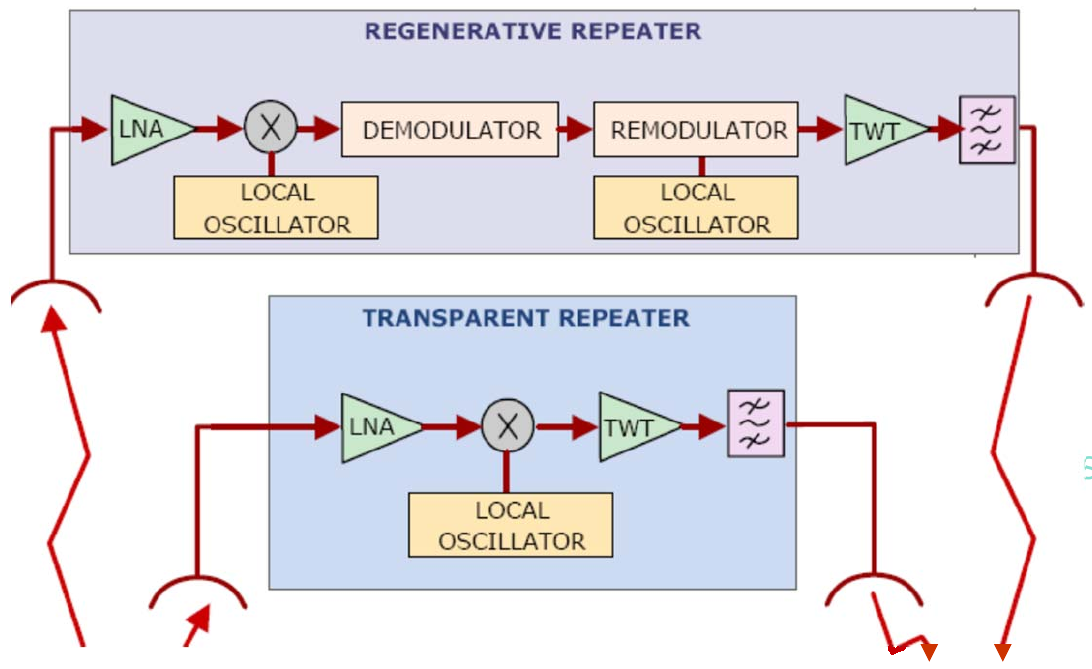
\includegraphics[
		width=14cm,
		%height=15cm
	]{images/Tema 5/Transponder.png}
	\caption{
		\label{fig:unit5_transponder}
		Transponder
	}
\end{figure}

\subsubsection{Antenna}

There are two types of antennas for satellites:
\begin{itemize}
	\item Wire (monopoles, dipoles): Used for TTC omni-directional.
	\item Horns (wide beam, global coverage).
	\item Reflectors (narrow beam).
	\item Arrays.
\end{itemize}

The most interesting ones are aperture antennas, whoch are horns and reflectors.

Main parameters are:

\begin{itemize}
	\item Antenna diameter: $D$
	\item Wavelength: $\lambda$
	\item {
		Aperture:
		$$
			A = \frac {\pi D^2} {4}
		$$
	}
	\item {
		Antenna gain:

		$$
			g = \eta \left( \frac {\pi D} {\lambda} \right)^2 = \eta \frac {4 \pi A} {\lambda^2}
		$$
		$$
			G = 10 \log (g)
		$$
	}
	\item {
		Beam width:
		$$
			\phi_{3dB} = \frac {70 \lambda} {D}
		$$
	}
\end{itemize}

Provided coverage can be:
\begin{itemize}
	\item Omni-directional.
	\item Global.
	\item Half-hemisphere.
	\item Beams.
\end{itemize}

\subsubsection{Multiple access}

Each EGSE owns a terminal for signal processing, modulation and transmission. It accesses to satellite in the uplink. The downlink is usually broadcast and each station extracts signal addressed to it. The satellite transponds the signal, amplifies it and filters it. Signal are multiplexed into the OMUX.

There are two techniques widely used:
\begin{itemize}
	\item {
		FDMA: The bandwidth is divided for all the active stations. Different carriers and guard bands are used for low mutual interference. At the satellite, the transponder converts the frequencies and amplifies them, causing the problem of inter-modulation noise at the amplifier.

		The satellite broadcasts the whole band. The receivers usually are wideband and receive the whole band and then tune only the one addressed to it. The narrowband stations only tunes a single channel carrier.

		In countries with low density in traffic, 12 channels are too much. So we use:
		\begin{itemize}
			\item Single Channel per Carrier (SCPC): A transponder per satellite.
			\item Demand Assigned Multiple Access (DAMA): Also used in TDMA.
		\end{itemize}

		FDMA has an easy implementation (only frequency modulation is needed and strict timing is not required.
	}
	\item TDMA: In TDMA, information must be digital. The avoidance of collisions is a must. Guard times are defined to avoid interference (arrival times of each station are not the same). There are dead times of 100 ns - 200 ns.
	\item {
		The TDMA is only used in the uplink, where the satellite receives all the frames from terminals and transmits by multiplexing them in time. There are one or two reference stations for TDMA. They do not carry traffic:
		\begin{itemize}
			\item Access control to the satellite.
			\item Synchronization.
		\end{itemize}
	}
	\item The number of slots per frame is between 3 and 100, and duration frames are between 125 $\mu s$ and 10 $ms$.
	\item In TDMA. all available power can be used, dynamic slot time adjustment provides flexibility for variable traffic and digitalness allows error control and digital modulations, but a strict timing required and there is an added delay due to discontinuous transmission.
\end{itemize}

\subsubsection{Link budget}

Link budget measures the contribution of all the powers, gains and losses involved in the link. It allows to estimate the link quality.

\begin{figure}[H]
	\centering
	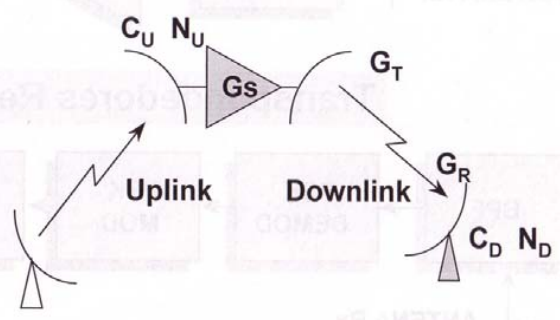
\includegraphics[
		width=7.5cm,
		%height=15cm
	]{images/Tema 5/Link budget.png}
	\caption{
		\label{fig:unit5_link_budget}
		Link budget
	}
\end{figure}

Two steps must be followed to obtain link budget:
\begin{itemize}
	\item {
		Calculate the available received power at receiver input and the noise density. The link has two sides, an uplink and a downlink with different $\left( \frac {C} {N} \right)_{up}$ and $\left( \frac {C} {N} \right)_{down}$:
		\begin{itemize}
			\item {
				General:
				$$
					\left( \frac {C} {N_0} \right)_{dB} = EIRP + \left( \frac {G} {T} \right) - L_{bf} - 10 \log(K) - BO [dBHz]
				$$
				$$
					\left( \frac {C} {N} \right)_{dB} = EIRP + \left( \frac {G} {T} \right) - L_{bf} - 10 \log(KB) - BO [dBHz]
				$$
			}
			\item {
				Uplink link budget:
				$$
					\left( \frac {C} {N_0} \right)_{dB, up} = EIRP_{sta} + \left( \frac {G} {T} \right)_{sat} - L_{bf, up} - 10 \log(K) - IBO [dBHz]
				$$
				$$
					\left( \frac {C} {N} \right)_{dB, up} = EIRP_{sta} + \left( \frac {G} {T} \right)_{sat} - L_{bf, up} - 10 \log(KB) - IBO [dB]
				$$
			}
			\item {
				Downlink link budget:
				$$
					\left( \frac {C} {N_0} \right)_{dB, down} = EIRP_{sat} + \left( \frac {G} {T} \right)_{sta} - L_{bf, down} - 10 \log(K) - OBO [dBHz]
				$$
				$$
					\left( \frac {C} {N} \right)_{dB, down} = EIRP_{sat} + \left( \frac {G} {T} \right)_{sta} - L_{bf, down} - 10 \log(KB) - OBO [dB]
				$$
			}
			\item {
				Total:
				$$
					\left( \frac {C} {N_0} \right)_{total}^{-1} = \left( \frac {C} {N_0} \right)_{up}^{-1} + \left( \frac {C} {N_0} \right)_{down}^{-1}
				$$
			}
		\end{itemize}
	}
	\item {
		Verify if the required quality criteria is accomplished. Some possible criteria are:
		\begin{itemize}
			\item Carrier to Noise Ratio: $\frac {C} {N} [dB]$
			\item Spectral Noise density: $N_0 [dB/Hz]$, $n_0 [W/Hz]$
			\item Equivalent Isotropic Radiated Power: $EIRP [dBW]$
			\item Gains: $G_{rx}, G_{tx} [dB]$
			\item Wavelength: $\lambda$
			\item Distance to satellite: $d$
			\item Bandwidth: $B [Hz]$
			\item Losses (atmospheric, polarization, depointing antennas, \ldots): $L [dB]$
			\item {
				Equivalent System Temperature:

				$T = T_a + T_0 (F_t - 1) [K]$
			}
			\item Noise antenna temperature: $T_0 = 290 [K]$, $T_a$
			\item Receiver Noise Figure: $F_t$
			\item Merit factor at receiver: $\frac {G} {T} [dB/K]$
			\item Energy per bit: $E_b (J/b, W/b)$
			\item Binary data rate: $R_b [b/s]$
			\item Input/Output Backoff: $IBO [dB]$, $OBO [dB]$
		\end{itemize}
	}
\end{itemize}

If the noise is uniformly distributed within the bandwidth ($B$), then $N = N_0 \cdot B$.

\section{Very Small Aperture Terminals (VSAT) services}

\subsection{Introduction}

VSAT networks a allow the implementation of Fixed Satellite Service (FSS) with small user terminals. They provide connection between remote terminals and the central HUB.

Main VSAT advantages are:
\begin{itemize}
	\item Connection in all points.
	\item High quality and availability.
	\item Easy network growth.
	\item Adapted to each traffic.
	\item Low implementation and exploitation.
\end{itemize}

\subsection{Elements}

VSAT networks are implemented with the following elements:
\begin{itemize}
	\item Network Control Center (NCC).
	\item Hub.
	\item Remote Terminal Units (RTU).
\end{itemize}

\begin{figure}[H]
	\centering
	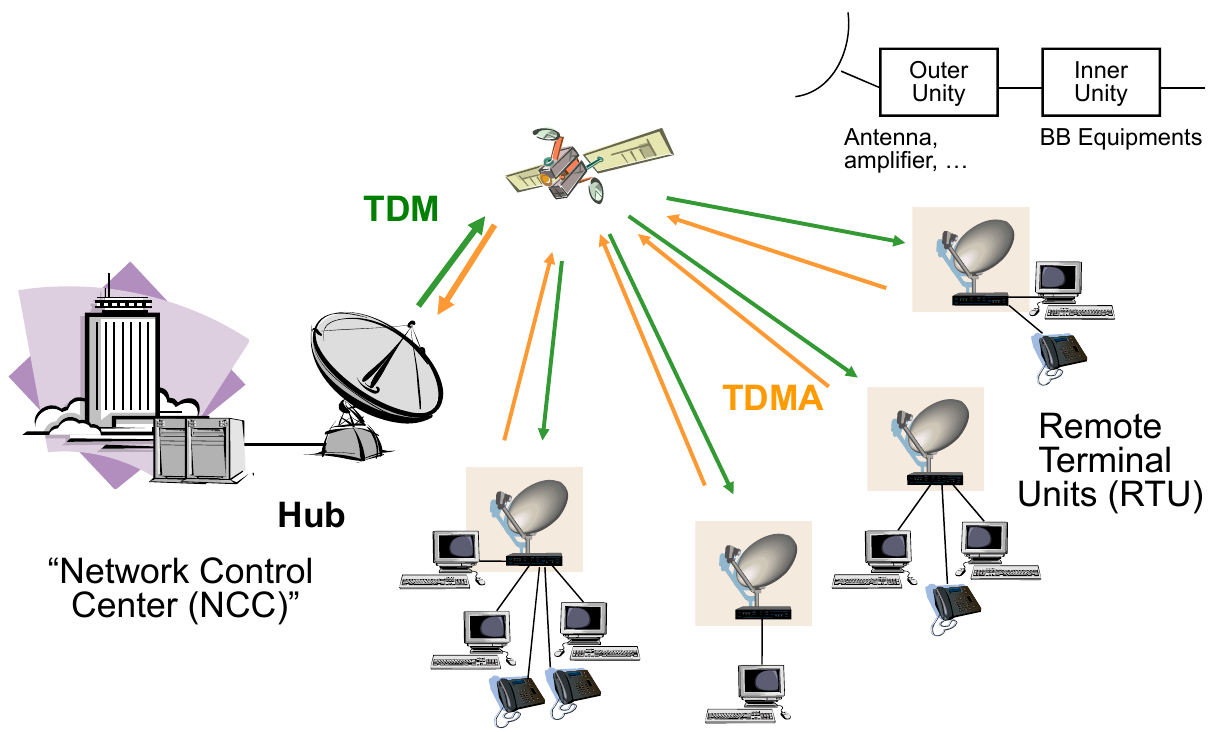
\includegraphics[
		width=14cm,
		%height=15cm
	]{images/Tema 5/VSAT elements.png}
	\caption{
		\label{fig:unit5_VSAT}
		VSAT elements
	}
\end{figure}

\subsection{Multiple access}

Multiple access is required at the inbound, but at RTU-S-RTU link (250 ms) multiple access can not be accomplished by carrier detection (TDM/TDMA).

Several possibilities are studied:
\begin{itemize}
	\item Random Access (RA/TDMA): For short burst traffic. It uses Aloha and S-Aloha.
	\item Demand Assignment (DA/TDMA): Continuous traffic. It uses Demand Assigned Multiple Access (DAMA) and R-Aloha (Aloha with reservation capacity). In DAMA, there are a channels pool and when a VSAT requests transmission, it ask for a channel and the HUB allocates it. These channels can be TDMA or FDMA.
	\item Fixed Assignment (FA/TDMA): Continuous traffic. A slot is exclusive allocated.
\end{itemize}

\section{Mobile satellite communications}

For mobile communication purposes, GEO and LEO are the preferred orbits. Tundra and Molniya are not used in PCS.

\begin{tabular}{|l|l|l|}
	\hline
							& GEO						& LEO \\
	\hline
	Number of satellites	& Three or four				& Between 40 and 100 \\
	\hline
	Delay					& 250 ms					& Few ms \\
	\hline
	Doppler shift			& 0							& Large \\
	\hline
	Elevation				& $10^{\circ} - 90^{\circ}$					& $10^{\circ} - 90^{\circ}$ \\
	\hline
	Satellite				& Big and complex			& Small \\
	\hline
	Earth segment			& Large, simple operation	& Small, complex operation \\
	\hline
	Coverage				& Not at poles				& Global \\
	\hline
	Handover time			& Hours or never			& Few minutes \\
	\hline
	Total cost				& Low						& High \\
	\hline
\end{tabular}

\section{Satellite navigation systems}

Satellite system for navigation purposes is very useful in landing and Required Navigation Performance (RNP) procedure.

\subsection{Global Positioning System (GPS)}

From the distance from three satellites to the receiver. Since the satellites positions are known, three spheroids can be calculated. The intersection among all of them gives the position. Since there are inherent measurement errors and clocks imprecision, pseudo-distances are calculated instead, being $R$ the real distance, $R'$ the pseudo-distance and $\epsilon$ the clock error due to drift. With 4 satellites, the clock deviation is also estimated. Thus:

$$
	R' = R + \epsilon = R + c \cdot \tau
$$

There are many source of errors (distance, clocks, propagation, \ldots). The propagation effect due to ionosphere can be corrected with the adequate model and measurement. It has been shown that:

$$
	R_m = R' + \frac {A} {f^2}
$$

Where $A$ is the ionosphere parameter that depends on its conditions.

\subsection{Galileo}

Galileo is a satellite navigation system proposed by the European Union with the support of European Space Agency (ESA) and a group of private investments.

The Galileo project is designed for civil uses. It had an estimated cost of 3 000 000 000 euros. Now it has increased in more than 4 000 000 000 euros. It was expected to be operational in 2008, then was delayed to 2011 - 2014, 2016.

Galileo is a GPS-independent system, but completely compatible and interoperable with it. A Galileo receiver will be able to exploit simultaneously received signals from Galileo satellites and GPS satellites (high number of satellites).

The specifications of Galileo space segment are:
\begin{itemize}
	\item Approximate weight of 600 kg.
	\item Payload of 110 kg.
	\item Power consumption of 1.7 kW.
	\item Higher power signal received. Thus, more difficult to be interfered.
	\item Rubidium-based clocks, much more stables. Nanoseconds precision.
\end{itemize}



\end{document}
